\documentclass[fleqn]{scrbook}
\usepackage[latin1]{inputenc}
\usepackage{latexsym}
\usepackage[german]{babel}
%\usepackage{ngerman}
\usepackage[a4paper]{geometry}
\usepackage[sumlimits]{amsmath}
\usepackage{graphicx}
\usepackage{pst-all}
\usepackage{multido}
\usepackage{glossar}
\usepackage{expdlist}
%\usepackage{nomencl}
\pagestyle{headings}
\usepackage{color}
\usepackage{keyval}
\usepackage{listings}
% Gleitobjekte erst nach Definition einf�gen
%\usepackage{flafter}
%\usepackage{charter}
%\geometry{textwidth=17cm, textheight=22cm} 
\parindent0em
\pagenumbering{arabic}

\renewcommand{\glshead}{\chapter*{Glossar}}


\newcommand{\todo}[1]{\hspace{0.5cm}\textbf{\textcolor{red}{TODO}: #1}\hspace{0.5cm}}

\newenvironment{notizen}
{%


\textbf{\textcolor{blue}{Notizen:}}\newline\textbf{\textcolor{blue}{$|^{---}$}}\begin{quote}
}%
{%
  \end{quote}
  \textbf{\textcolor{blue}{$|_{---}$}} \newline
}%

\makeatletter
% args are: width,height,caption,label
\newcommand{\picturehere@caption}{false}
\newcommand{\picturehere@label}{false}
\define@key{picturehere}{caption}[false]{
  \renewcommand{\picturehere@caption}{#1}}
\define@key{picturehere}{label}[false]{
  \renewcommand{\picturehere@label}{#1}}
\newenvironment{picturehere}[4]%
{%
 \setkeys{picturehere}{caption = #3, label = #4}
  \begin{figure*}[h]%
    \begin{center}%
      \begin{minipage}[b]{.3\linewidth}%
        \psset{xunit=1cm,yunit=1cm,runit=1cm}%
        \begin{pspicture}(#1,#2)%
}%
{%
        \end{pspicture}%
      \end{minipage}%
    \end{center}%
    \caption{\picturehere@caption}%
    \label{\picturehere@label}%
  \end{figure*}%
}
\makeatother

\newcommand{\importgnuplotps}[3]{
  \begin{picturehere}{1}{10}{\mbox{#1}}{#2}
    \includegraphics[bb=530 310 730 600,scale=0.55,angle=-90]{#3}
  \end{picturehere}
}

\newcommand{\importsmallgnuplotps}[3]{
  \begin{picturehere}{1}{7}{\mbox{#1}}{#2}
    \includegraphics[bb=530 310 730 600,scale=0.4,angle=-90]{#3}
  \end{picturehere}
}

\newcommand{\pubsubrss}{Pub/Sub-RSS }



\includeonly{einleitung,grundlagen,rss_mittels_verteiltem_pubsub,adaptive_informationsverteilung,experimente,anhang,glossar}

%\title{Adaptive Informationsverbreitung mittels RSS und Publish/Subscribe \\[2cm]\textnormal{Diplomarbeit}}
%\author{Friedemann Zintel}
%\date{\today}

\begin{document}
%\sffamily

%\maketitle

\bibliographystyle{alpha}
%\bibliographystyle{plain}

\frontmatter

\begin{titlepage}
  \begin{center}
    \vspace*{2.5cm}
     \textbf{{\LARGE Diplomarbeit}}\par
    \vspace{1.25cm}
    {\linespread{1.85}\selectfont \textsf{\textbf{{\huge Adaptive Informationsverbreitung mittels RSS und Publish/Subscribe}}}\par}
    \vspace{2.25cm}
    \textnormal{{\Large Friedemann Zintel}}\par
    \vspace{0.75cm}
    {\Large \today}
    \newpage
    \vspace*{4cm}
    \textnormal{{\Large Hiermit versichere ich, den Text eigenst�ndig verfasst zu haben.}}
  \end{center}
\end{titlepage}

\setcounter{tocdepth}{2}
\setcounter{secnumdepth}{2}
\tableofcontents
\listoffigures
\listoftables

\mainmatter

\chapter{Einleitung}
\section{Motivation}
\section{Ziel der Arbeit}
\section{Aufbau der Arbeit}

\chapter{Grundlagen}
\label{Abschnitt:Grundlagen}
In diesem Kapitel sollen einige Begriffe und Verfahren erkl�rt werden, die f�r das Verst�ndnis des weiteren Textes notwendig erscheinen.
\section{Peer-To-Peer-Systeme}
\section{Publish/Subscribe-Systeme}
\label{publishsubscribe}
\subsection{Filter}
%\section{Andere Arbeiten}
%%% Local Variables: 
%%% mode: latex
%%% TeX-master: "diplomarbeit"
%%% End: 

\section{Timer}
\label{css:timer}
Ein wichtiger Bestandteil der im weiteren Verlauf der Arbeit vorgestellten Verfahren sind Timer. Daher stellen wir
zun�chst dar, was unter dem Begriff ``Timer'' zu verstehen ist und welche Problematiken sich im Umgang mit Timern ergeben.\\

Bei der Kommunikation zwischen Computern werden Informationen im allgemeinen in einzelne Datenpakete eingeteilt und zwischen
den beteiligten Computern ausgetauscht. Ein Timer ist ein Mechanismus, um in Computer-Kommunikationsnetzen Fehler erkennen zu k�nnen \cite{18216},
welche bei der Kommunikation zwischen Computern auftreten. Diese Fehler k�nnen im einzelnen Verluste von Datenpaketen, das Zusammenbrechen
von Kommunikationskan�len oder indirekt eine Verst�mmelung der �betragenen Informationen bezeichnen. Dabei arbeitet ein Timer wie eine Alarm-Uhr:
nach einer vordefinierten Zeit l�uft der Timer ab. In der Annahme, dass ein bestimmtes Ereignis innerhalb dieser
vordefinierten Zeit zu geschehen hat (im Regelfall eine Antwort des Kommunikationspartners), deutet ein abgelaufener Timer auf
einen aufgetretenen Fehler hin. Hierbei ergeben sich erste Probleme: ist die Zeitspanne bis zum Ablauf eines Timers zu lang,
so wird ein eventuell aufgetretener Fehler zu sp�t erkannt. Ist die Zeitspanne dagegen zu kurz, so kann dies einen falschen Alarm zur Folge haben.
Um ein optimales Leistungsverhalten zu erzielen, wird ein Gleichgewicht zwischen diesen gegens�tzlichen Zielen angestrebt.\\

Verschiedene Timer werden bei Kommunikationsprotokollen (Bsp. TCP, siehe Abschnitt \ref{staukontrolle_tcp}) verwendet, um verschiedenartige
Formen der Kommunikationsst�rung zu erkennen. So sorgt ein ``retransmission-timer'' f�r das wiederholte Aussenden von eventuell verloren gegangenen
Datenpaketen. Dagegen gibt ein ``death-timer'' Auskunft �ber den Zusammenbruch einer Datenverbindung \cite{18216}. Die Zeitspannen
(``Timeout-Intervalle'') werden dabei je nach Timer unterschiedlich gesetzt. Um ein Gleichgewicht zwischen der Reduzierung falscher Alarme
und der rechtzeitigen Erkennung aufgetretener St�rungen zu erreichen, werden die Timeout-Intervalle meistens dynamisch und situationsabh�ngig
bestimmt. Folgende Situationen k�nnen nach Zhang \cite{18216} beispielsweise f�r das Ablaufen von retransmission-timern urs�chlich sein:
\begin{enumerate}
\item Ein Datenpaket hat den den Sender noch nicht verlassen (aufgrund eines beispielsweise blockierten Netzwerks), befindet sich aber bereits
  in einer tieferen Anwendungsschicht.
\item Das Timeout-Intervall ist k�rzer als die Zeit bis zu einer positiven Antwort vom Empf�nger.
\item Ein Datenpaket hat den Empf�nger erreicht, die Best�tigungsnachricht ging jedoch verloren.
\item \label{En:Congestion} Ein Datenpaket wurde an einem Vermittlungsknoten (Gateway) aufgrund von Datenstau verworfen.
\item \label{En:Channelerror}Ein Datenpaket wurde augrund eines Fehlers im �bertragungskanal verworfen.
\item Das Netzwerk wurde partitioniert oder der Empf�nger-Knoten ist ausgefallen.
\end{enumerate}

Nur bei Punkt \ref{En:Channelerror} ist ein unmittelbares und wiederholtes Aussenden notwendig. Punkt \ref{En:Congestion} erfordert zwar
auch ein wiederholtes Aussenden eines Datenpakets, das Setzen des retransmission-timers muss aber mit Bedacht geschehen,
um den urs�chlichen Datenstau nicht noch zu vergr��ern. Zhang beschreibt in \cite{18216} die Problematik bei dynamischer Bestimmung der
Timeout-Intervalle. Techniken zur dynamischen Bestimmung von Timeout-Intervallen werden wir in Abschnitt \ref{staukontrolle_tcp} vorstellen.


 
%%% Local Variables: 
%%% mode: latex
%%% TeX-master: "diplomarbeit"
%%% End: 

\section{Staukontrolle bei TCP}
\label{staukontrolle_tcp}
Seitdem Computer-Netzwerke explosionsartig an Gr��e und Komplexit�t zugenommen haben, hat sich ein Problem verst�rkt bemerkbar gemacht: Datenstau.
Van Jacobson et. al. \cite{jacobson88congestion} schildern die Beobachtung, dass Mitte der 1980er Jahre Internet-Gateways 10\% der
ankommenden Pakete aufgrund von Puffer�berl�ufen verwarfen. Laut seiner Aussage lag dabei das Problem nicht in den Protokollspezifikationen selbst, sondern
haupts�chlich in deren Implementierungen. TCP ist ein verbindungsorientiertes �ber\-tra\-gungs\-pro\-to\-koll, mit dessen Hilfe der Gro�teil
des Netzwerkverkehrs vonstatten geht. Im Laufe der Zeit wurden in TCP Mechanismen eingebaut und verbessert, um Datenstau festzustellen und soweit wie m�glich
zu vermeiden. TCP kontrolliert die Daten�bertragung zwischen Sender und
Empf�nger der Endknoten. Dabei wird gew�hrleistet, dass jedes der einzelnen Datenpakete (die einen Datenstrom formen) den Empf�nger erreicht
und dass die Ordnung der Pakete
innerhalb des Datenstroms bestehen bleibt. Bei Datenstau handelt es sich um Verlust von Datenpaketen. Falls es zu Datenstau kommt, so tritt dieser immer an
Verbindungsknoten (einschlie�lich des Empfangsknotens) auf und kann durch verschiedene Ursachen auf dem Weg zwischen Sender und Empf�nger hervorgerufen werden:
\begin{description}
  \item [Bandbreiten:]
    Unterschiedliche Bandbreiten auf dem Weg zwischen Sender und Empf�nger beeinflussen die �bertragungsgeschwindigkeit einer Verbindung
    nachteilig in der
    Form, dass die ``langsamste'' Leitung (also die mit der geringsten Bandbreite) die
    Gesamt-�bertragungsgeschwindigkeit vorgibt. Trifft eine schnelle Leitung auf eine langsame Leitung, so k�nnen die an der langsamen Leitung ankommenden
    Pakete nicht schnell genug weitergeleitet werden. An diesem Knoten kommt es zum Puffer�berlauf, Datenpakete gehen verloren.
  \item [Anzahl der Verbindungen:]
    An einem Knotenpunkt k�nnen mehrere Verbindungen zusammen kommen, die den Gesamt-Datenfluss an diesem Punkt erh�hen. Auch hier kann es zum Puffer�berlauf
    kommen, so dass Datenpakete verloren gehen.
\end{description}
Damit jedes ausgesandte Paket den Empf�nger erreicht, werden in TCP Best�tigungs-Nachrichten (Acknowledgements, im Folgenden kurz $acks$ genannt) versandt.
Erh�lt der Sender f�r ein gesendetes TCP-Datenpaket kein $ack$, so wird er das Datenpaket erneut senden. Ein wichtiger Bestandteil eines Datenpaketes ist
die Sequenznummer \cite{RFC2581}. Anhand der Sequenznummer kann ein $ack$ eindeutig einem versendeten Datenpaket zugeordnet werden. Innerhalb des $acks$ vermerkt
der Empf�nger ebenfalls, welches Datenpaket er als n�chstes erwartet \cite{RFC793}.
Um eine Staukontrolle zu erreichen wurden einige Algorithmen in TCP integriert (siehe \cite{jacobson88congestion}, wir halten uns dabei an die englischen
Bezeichnungen):
\begin{itemize}
  \item slow-start
  \item roundtrip-time variance estimation
  \item exponential retransmit timer backoff
  \item more aggressive receiver ack policy
  \item dynamic window sizing on congestion
  \item Karn's clamped retransmit backoff
  \item fast retransmit
\end{itemize}

Dabei soll erreicht werden, dass die maximal m�gliche Bandbreite (begrenzt durch die minimale Bandbreite (``bottleneck'') auf dem Verbindungsweg, s. o.) voll
ausgenutzt wird, ohne
dass Pakete verloren gehen; es darf also kein Paket in das Netzwerk eingespeist werden, bevor ein altes Paket entfernt wurde (die Verbindung befindet sich dann im
``Equilibrium'', der Paketfluss ist ``conservative'' \cite{jacobson88congestion}). Im Folgenden wollen wir die wichtigsten der oben genannten Algorithmen
vorstellen. Eine genaue Herleitung und Analyse der Algorithmen geht jedoch �ber den Rahmen dieser Arbeit hinaus.
Wir verweisen auf die entsprechenden Quellen in den Literaturangaben.

\paragraph{more aggressive receiver ack policy:}
\footnote{Hier ist in \cite{jacobson88congestion} nicht eindeutig feststellbar,  worauf sich van Jacobson genau bezieht, da er diese Bezeichnung im weiteren Text
nicht mehr verwendet. Es erschien sinnvoll, die folgende im o. g. Text zu findende Erkl�rung diesem Thema zuzuordnen.}TCP
ist ``self-clocking'': da $acks$ erst nach Erhalt der entsprechenden Datenpakete versendet werden k�nnen, bestimmt die Rate der ankommenden $acks$ die
Rate, mit der weitere Datenpakete ausgesendet werden sollen. Die Senderate passt sich somit automatisch der Bandbreite an.

\paragraph{slow-start:}
Durch das ``self-clocking'' tritt nur beim Start des Datentransfers ein Problem auf, da
hier zun�chst eine feste Rate gew�hlt werden muss. Diese wird zu Beginn relativ niedrig gew�hlt, bzw. ein Staufenster ``congestion window'' ($cngw$) 
bestimmt die Anzahl der Pakete pro Sendevorgang. Bei Start des Transfers oder nach Paketverlust wird die Gr��e des Staufenster auf 1 gesetzt.
F�r jedes $ack$ wird das Staufenster um den Betrag 1 erh�ht. Begrenzt wird dessen Gr��e durch das ``advertised receiver window'',
welches vom Empf�nger festgelegt wird und angibt, wieviele Bytes maximal als n�chstes �bersendet werden sollen. Die Zunahme der Gr��e $w$ des
Staufensters geschieht in der Zeit
$rtt\cdot log_2w$, wobei $rtt$ die ``roundtrip-time'' des letzten versendeten Datenpaketes ist (Zeit zwischen Versenden eines Datenpaketes und Erhalt des
entsprechenden $acks$). Siehe dazu \cite{jacobson88congestion,RFC2581}. 

\paragraph{roundtrip-time variance estimation:}
\label{cssp:tcp_rtt}
$Acks$ k�nnen die Geschwindigkeit des Datenflusses steuern, doch was geschieht, wenn $acks$ aufgrund verloren gegangener Pakete ausbleiben? M�ssen sich
beispielsweise bei voll ausgenutzter Bandbreite pl�tzlich zwei Datenstr�me dieselbe Leitung teilen, kommt es bei gleichbleibender Datentransferrate mit Sicherheit zu
Paketverlusten und somit zu
ausbleibenden $acks$. Der Sender muss einen Timer unterhalten, bei dessen Ablauf das zuletzt gesendete Datenpaket erneut versendet wird (im Folgenden als
``Wiederholung'' bezeichnet). Paketverlust kann auch
durch Besch�digung der Daten w�hrend der �bermittlung auftreten. Nach van Jacobson \cite{jacobson88congestion} liegt die Wahrscheinlichkeit daf�r aber weit
unter 1\%. Daher lassen Timeouts bei gut eingestellten Timern mit sicherer Gewissheit auf Paketverluste schlie�en \footnote{Zur Problematik
bei Timern siehe \ref{css:timer}}. Diese Timeouts werden pro Verbindung dynamisch berechnet; im Folgenden bezeichnet $rto$ das ``retransmission timeout''-Intervall,
also die Zeitdifferenz bis zum n�chsten Aussenden eines Datenpaketes. Entsprechend der TCP-Spezifikation
berechnet sich dieser Wert wie folgt \cite{18216}:
\begin{equation}
  rto=min\{UBound, max\{LBound, \beta \cdot srtt\}\}
\end{equation}
$\beta$ ist dabei ein empirisch ermittelter Varianz-Faktor, $UBound$ und $LBound$ sind untere und
obere Schranke f�r den $rto$, $srtt$ ist die ``smoothed roundtrip time'' und
wird wie folgt ermittelt:
\begin{equation}
  srtt= \alpha \cdot  srtt+ (1 - \alpha) \cdot  rtt
\end{equation} 
$\alpha$ ist ein ebenfalls empirisch ermittelter Gl�ttungsfaktor (``smoothing factor''). Empfohlene Werte sind f�r $\alpha:$ $0.8 \sim 0.9$ und f�r $\beta:$
$1.3 \sim 2$ \cite{18216}.\\
Laut van Jacobson \cite{jacobson88congestion} liegt hierin folgende Problematik: $\beta$ kann sich h�chstens an eine bis zu 30\% gesteigerte Last anpassen. Aber die
Varianz des Wertes $rtt$ steigert sich rapide mit ansteigender Last. Bei
Laststeigerung �ber die 30\%-Marke hinaus kommt es zu versp�teten $acks$. Der jeweilige abgelaufene Timer bewirkt eine Wiederholung des entsprechenden
Datenpaketes, was zu unn�tiger Mehrarbeit des Netzwerkes und zu Bandbreitenverschwendung f�hrt. Daher wird $\beta$ ebenfalls dynamisch berechnet.
Eine Berechnungsmethode findet sich in \cite{jacobson88congestion}.

\paragraph{exponential retransmit timer backoff:}
Um den Datenstau durch mehrfach ausgesandte Pakete nicht noch zu vermehren, muss sich der $rto$ stetig vergr��ern.
Van Jacobson \cite{jacobson88congestion} stellt heraus, dass nur exponentielles Wachstum des $rto$ Erfolg verspricht.
Daher wird nach jedem erneuten Aussenden eines nicht best�tigten Datenpaketes der $rto$ verdoppelt.

\paragraph{dynamic window sizing on congestion:}
Ein Vergr��ern des $rto$ verhindert nur einen zus�tzlichen Datenstau durch erneut ausgesandte Datenpakete. Damit auch die im Anschluss daran neu
ausgesandten Pakete nicht wieder zum Anstieg des Datenstaus f�hren, wird ebenfalls die Gr��e der Staufenster $cwnd$ halbiert (exponentielle Abnahme).
Ausbleibende oder verz�gerte $acks$ geben nur Auskunft �ber auftretenden Datenstau. Sie k�nnen nicht anzeigen, ob die volle Bandbreite einer Verbindung auch wirklich
ausgenutzt wird. Daher sollte die Gr��e der Staufenster nach einem bestimmten Schema angehoben werden. Die Anpassung von $cwnd$ geschieht nach folgendem Prinzip:
\begin{itemize}
  \item Nach jedem Timeout wird $cwnd$ halbiert.
  \item Nach jedem $ack$ f�r neue Daten wird $cwnd$ um $1/cwnd$ erh�ht.
  \item Beim Senden wird das Minimum an Daten von $cwnd$ und dem ``receivers advertised window'' gesendet.
\end{itemize}

Dieser Algorithmus tr�gt zur Stauvermeidung (``congestion avoidance'') bei und besteht parallel zum ``slow-start''-Algorithmus. Van Jacobson gibt in
\cite{jacobson88congestion} ein Auswahlkriterium an, nachdem zustandsabh�ngig zwischen beiden Algorithmen ausgew�hlt wird.

\paragraph{Karn's clamped retransmit backoff:}
\label{csp:karns_algorithmus}
Sequenznummern erm�glichen die Zuordnung eines $acks$ zu dem entsprechenden Datenpaket. Kommt es aufgrund von Timeouts zu Wiederholungen
desselben Datenpaketes, so tritt ein Problem auf, welches Karn und Partridge in \cite{Karn1991} als ``retransmission ambiguity'' bezeichnen:
es kann nicht festgestellt werden, auf welche Aussendung desselben Datenpaketes sich das $ack$ bezieht. Damit ist nicht klar, anhand welches Paketes
sich der $rtt$ bestimmen soll, er wird in jedem Falle nicht verl�sslich sein. Verschiedene Protokollimplementationen behandeln dieses Problem
auf unterschiedliche Weise: teils wird die am l�ngsten zur�ckliegende Aussendung als Grundlage zur Berechnung herangezogen, teils die am k�rzesten zur�ckliegende
Aussendung.\\

Wird die am l�ngsten zur�ckliegende Aussendung  gew�hlt, so k�nnen der $rtt$, damit der $srtt$ und letztlich der $rto$ unverh�ltnism��ig in die H�he schie�en.
In vielen F�llen ist die nachteilige Wirkung nicht besonders gro�, da aufgrund des Datenstaus eine Drosselung der Datentransferrate erw�nscht ist.
Kommt es aufgrund anderer Ursachen zu Paketverlusten (z. B. bei verlustreichen Leitungen durch St�rsignale), so tritt das Gegenteil des gew�nschten Verhaltens
ein: der $srtt$ sinkt auf ein sehr niedriges Niveau, obwohl sich in diesem Falle die Datentransferrate erh�hen sollte.\\

Wird die am k�rzesten zur�ckliegende Aussendung herangezogen, so ist die Wahrscheinlichkeit laut Karn sehr gro�, dass die Zeitfolge zwischen dieser Sendung und dem
ankommenden $ack$ sehr kurz ist, obwohl sich das $ack$ auf eine weiter zur�ckliegende Sendung bezieht. Dies f�hrt zu einer drastischen Reduzierung des $srtt$,
was �berfl�ssige Wiederholungen und damit eine zus�tzliche Verschwendung der Bandbreite zur Folge hat \cite{Karn1991,Jain1986}. Andere Implementationen
lassen den $rtt$ bei Wiederholungen au�er acht. Dies geht gut, solange der $rto$ nicht schneller ansteigt, als der Algorithmus sich adaptieren kann. Ist $\beta$
gut gew�hlt, so ist die M�glichkeit daf�r sehr gering. Tritt dieser Fall dennoch ein, so kommt es (wie im letztgenannten Fall) zu �berfl�ssigen Wiederholungen.\\

Um diesem Problem zu begegnen, schl�gt Karn folgenden Algorithmus vor \cite{Karn1991}:\\
Grunds�tzlich wird der $rto$ nach einem Timeout vergr��ert (``back-off'').
Erreicht ein $ack$ den Sender nach einer Wiederholung eines Datenpaketes, so wird keine Neuberechnung des $rtt$ und $srtt$ vorgenommen. Daf�r wird der neu
ermittelte (``backed-off'') $rto$ als Grundlage f�r die n�chste Wiederholung bzw. f�r die Aussendung des n�chsten Datenpaketes herangezogen. Nur wenn ein $ack$
den Sender ohne vorausgehende Wiederholung erreicht, wird der $rto$ mit Hilfe des nun neu berechneten $srtt$ ermittelt.\\
Die Wahl des neuen $rto$ im Falle einer Wiederholung muss laut Karn so erfolgen, dass der $rto$ gr��er ist als die tats�chliche roundtrip-time. Typischerweise
geschieht die Steigerung des $rto$ exponentiell (entsprechend des ``exponential retransmit timer backoff'', s. o.).

\paragraph{fast retransmit:}
Erreichen den Sender vier identische $acks$ in Folge, so wird der Sender das vom Empf�nger erwartete Datenpaket sofort aussenden, ohne auf das
Ablaufen des Retransmission-Timers zu warten. ``Slow-start'' wird so lange ausgesetzt, bis ein anderes, nicht zu den vorherigen identisches $ack$ den Sender
erreicht  (\cite{RFC2581}). Die identischen $acks$ lassen sowohl darauf schlie�en, dass ein Datenpaket verloren gegangen ist, als auch, dass andere Datenpakete den
Empf�nger h�chstwahrscheinlich erreichen, da die identischen $acks$ sonst ausgeblieben w�ren. Die den identischen $acks$ zugrundeliegenden Datenpakete beeinflussen
das Datenaufkommen nicht mehr, da diese schon die Empf�nger-Queue erreicht haben. Daher geht man davon aus, dass das erneute, schnelle Senden des fehlenden
Datenpaketes das Netz nicht wesentlich im Negativen beeinflusst. ``Fast retransmit'' sollte, muss aber nicht, von einer konkreten TCP-Implementation unterst�tzt
werden.\\

Zus�tzliche Erweiterungen zum TCP in Hinsicht auf hohe Performanz finden sich in \cite{jacobson93tcp}.

%%% Local Variables: 
%%% mode: latex
%%% TeX-master: "diplomarbeit"
%%% End: 

\section{Regelkreise}
\label{regelungstechnik}
Auf dem Gebiet der Regelungstechnik besch�ftigt man sich damit, wie eine Gr��e einen bestimmten vorgegebenen Wert erreichen und halten kann. Bei einer Regelung
finden Kontrollmechanismen
Anwendung, um Wertabweichungen festzustellen und auszugleichen.\\

Die Aufgabe einer Regelung besteht darin, bestimmte Gr��en (Temperatur, Spannung, etc.) auf einen
vorgeschriebenen Wert zu bringen und diesen entgegen allen St�reinfl�ssen konstant zu halten (\cite{Bernstein1998}). Bei der Regelung unterscheidet man zwischen
verschiedenen Gr��en, die zusammen einen Regelkreis bilden: 
\begin{description}
  \item [Regelgr��e $x$] oder auch der Istwert: Gr��e, welche konstant gehalten werden soll und zu diesem Zweck erfasst wird
  \item [F�hrungsgr��e $w$] oder auch Sollwert: vorgegebener Wert, auf den die Regelgr��e eingestellt werden soll
  \item [St�rgr��e $z:$] Gr��e, die die Regelgr��e in unerw�nschter Weise beeinflusst
  \item [Regeldifferenz $x_d:$] Differenz zwischen F�hrungs- und Regelgr��e $x_d=w-x$
  \item [Stellgr��e $y:$] Gr��e, durch welche die Regelgr��e in erw�nschter Weise beeinflusst wird
\end{description}

\begin{picturehere}{1}{4}{Regelkreis}{Abb:Regelkreis}
 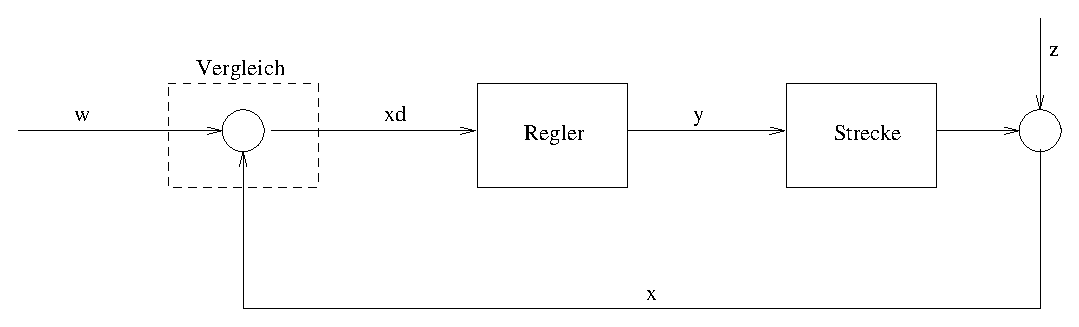
\includegraphics[bb=180 0 682 141,scale=0.75]{Regelkreis}
\end{picturehere}

%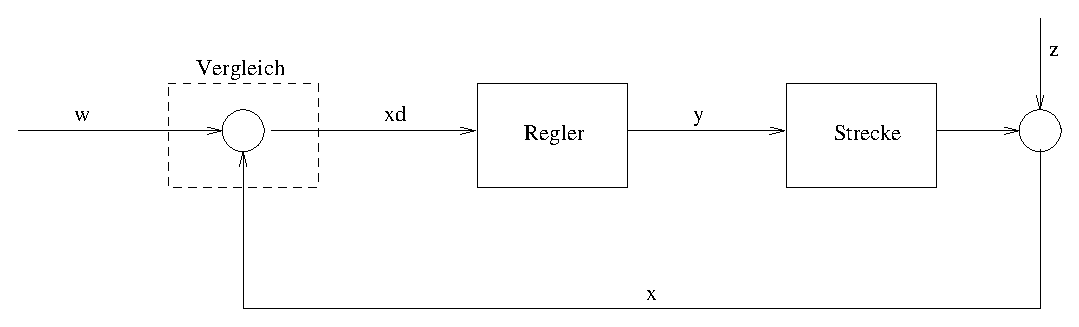
\includegraphics[scale=0.75]{Regelkreis.pstex}

Bild \ref{Abb:Regelkreis} zeigt das vereinfachte Schema eines Regelkreises. Die Regelung basiert auf R�ckkopplung. Bewirkt der Einfluss der St�rgr��e eine
Abweichung der Regelgr��e von der F�hrungsgr��e, so ergibt die Regeldifferenz �ber einen Regler eine Stellgr��e, die entgegengesetzt zur St�rgr��e auf die
Regelgr��e einwirkt. Ziel dabei ist es, die Regeldifferenz auf Null zu bringen.\\
Die Wahl eines geeigneten Reglers h�ngt stark von der Regelstrecke ab. Die Regelstrecke bezeichnet die zu regelnde Anlage oder den zu regelnden Prozess. Wichtig zu
wissen ist, wie die Regelstrecke auf �nderung der Einflussgr��en reagiert. Nach \cite{Bernstein1998} kann man die Regelstrecken grob durch folgende Merkmale 
unterscheiden:
\begin{itemize}
  \item Regelstrecken mit und ohne Ausgleich
  \item Regelstrecken mit und ohne Totzeiten bzw. Zeitgliedern
  \item lineare oder nichtlineare Regelstrecken
\end{itemize}

Bei Regelstrecken mit Ausgleich erreicht die Ausgangs- bzw. Regelgr��e nach einer gewissen Zeit einen stabilen Zustand (Bsp. Raumtemperatur). Existiert kein
stabiler Zustand (Regelstrecke ohne Ausgleich), so �ndert sich bei konstanter Eingangs- bzw. Stellgr��e die Regelgr��e mit
konstanter Geschwindigkeit oder Beschleunigung (Bsp. F�llen eines Wasserbeh�lters). Totzeit bezeichnet eine Zeitverz�gerung, bis sich die �nderung der Stellgr��e
auf die Regelgr��e bemerkbar macht. Bei linearen Regelstrecken folgt die Regelgr��e der Stellgr��e proportional.

Meist liegt eine Kombination dieser Eigenschaften vor. Um die Stellgr��e entsprechend der Regeldifferenz anzupassen, wird ein Regler ben�tigt.

\paragraph{PID-Regler:}
Ein PID-Regler ist ein allgemeiner Reglertyp, der h�ufig f�r Regelungen Verwendung findet. Er ist eine Kombination aus einem P-, einem I- und einem D-Regler.
Ein P-Regler sorgt daf�r, dass (im station�ren Zustand) ein dem Eingangssignal proportionales Ausgangssignal geliefert wird (unter Zuhilfenahme eines
Verst�rkungsfaktors). Ein I-Regler summiert die Regeldifferenz �ber einen gewissen Zeitraum und f�hrt damit eine Integration aus. Je l�nger eine Regeldifferenz
besteht, desto gr��er wird die Stellgr��e. Ein D-Regler reagiert nur auf die �nderungsgeschwindigkeit der Regeldifferenz. Er liefert einen entsprechend starken,
kurzen, positiven Impuls.

Die allgemeine mathematische Gleichung f�r einen PID-Regler lautet wie folgt
(siehe \cite{WBuettner1991}):
\begin{equation}
  u(t)=K_R\left[\quad e(t) \quad + \quad
    \frac{1}{T_I}\int\limits_{0}^{t}e(\tau)d\tau \quad + \quad
    T_D\frac{de(t)}{dt} \quad \right]
\end{equation}

Die einzelnen Gr��en sind:
\begin{description}
  \item [$u(t)$] Stellgr��e
  \item [$e(t)$] Regeldifferenz
  \item [$K_R$] Verst�rkungsfaktor
  \item [$T_I$] Integrationskonstante
  \item [$T_D$] Differentiationskonstante
\end{description}

Es werden nicht f�r alle Regelungen alle Anteile ben�tigt. Durch Weglassen der entsprechenden Anteile erh�lt man die Regler P, PI bzw. PD. Reine P-Regler finden
nur Verwendung bei Regelstrecken linearen Verlaufs. Doch selbst hier zeigt sich, dass bei Regelabweichungen, die durch eine St�rgr��e hervorgerufen werden, die
St�rgr��e lediglich in ihrer Wirksamkeit gemindert werden kann. Eine vollst�ndige Beseitigung tritt nicht ein, da die Regelabweichung selbst notwendig ist, um eine
Verstellung des Stellgliedes vorzunehmen \cite{Bernstein1998}. Mit einem I-Regler kann man die Regelabweichung sehr genau unterbinden, jedoch arbeitet dieser
relativ langsam und neigt zu Schwingungen. Die Vorteile beider Reglertypen vereint der PI-Regler. Reine D-Regler finden in der Praxis keine Verwendung, da sie bei
stabiler Regelgr��e nicht in den Regelvorgang eingreifen k�nnen. Die Kombination mit einem P-Regler (also ein PD-Regler) bewirkt ein schnelleres Anspringen der
Regelung bei pl�tzlicher Regelabweichung im Vergleich zu einem reinen P-Regler.

%%% Local Variables: 
%%% mode: latex
%%% TeX-master: "diplomarbeit"
%%% End: 


%%% Local Variables: 
%%% mode: latex
%%% TeX-master: "diplomarbeit"
%%% End: 

\chapter{RSS mittels verteiltem Publish/Subscribe}
\chapter{RSS}
\label{ch_rss}
%\subsection{Optionale Parameter}
\label{op_rss}

\subsection{Das Verteilungsschema}
Ein Problem bei Dienstapplikationen im Internet ist eine starke Serverbelastung zu gewissen Sto�zeiten.
Die Masse der Anfragen an einen Server kann dazu f�hren, dass dieser der zeitgerechten Beantwortung nicht mehr nachkommen kann.
Im schlimmsten Fall
k�nnen einige Anfragen gar nicht beantwortet werden, da die Masse der Anfragen die zur Verf�gung gestellte Speicherkapazit�t des Servers
�bersteigt. Ein Server unterh�lt im Regelfall eine Warteschlange (Queue) in der diejenigen Anfragen vorgehalten werden, welche aufgrund
anderer in Abfertigung befindlicher Anfragen momentan nicht bearbeitet werden k�nnen. Wird die Kapazit�tsgrenze dieser Warteschlange erreicht,
k�nnen weitere �bersch�ssigen Anfragen nicht bearbeitet werden, sie werden verworfen.
Beim bestehenden Konzept zur Verteilung der RSS-Feeds kann es
vorkommen, dass Subscriber, deren Anfragen sich sehr weit hinten in der Warteschlange befinden, erst sehr sp�t bzw. zu sp�t die gew�nschten
Informationen erhalten. Man denke z.B. an aktuelle B�rsennachrichten, welche im Sekundenbereich aktualisiert werden. Hier kann eine Nachricht
schon als veraltet gelten, erreicht sie den Interessenten einige Sekunden zu sp�t. Subscriber, deren Anfragen den Server bei bereits
ausgesch�pfter Kapazit�t der Warteschlange erreichen, kommen gar nicht an die gew�nschte Information.

Unser Ziel ist es, ein Verteilungsschema zu konzipieren, bei dem jeder Subscriber die gew�nschte Information in angemessener bzw.
gew�nschter Zeit erh�lt. Je fr�her ein Subscriber die neueste Information, die beim Server vorliegt, erh�lt, desto gr��er ist ihr Aktualit�tsgrad.
F�hren wir uns kurz vor Augen, welche Faktoren den Aktualit�tsgrad beeinflussen k�nnen. Denkbar sind drei Situationen, die den Aktualit�tsgrad
negativ beeinflussen:
\begin{enumerate}
  \item Anfrage des Subscribers an den Server kommt zu sp�t \label{enum:anf_zsp}
  \item Antwort des Servers erreicht den Subscriber zu sp�t \label{enum:ant_zsp}
  \item Subscriber erh�lt gar keine Antwort vom Server \label{enum:k_ant}
\end{enumerate}

Zu \ref{enum:anf_zsp}.: da wir es bei dem bestehenden Pull-Ansatz mit aktivem Polling der Subscriber zu tun haben, bewirkt eine h�here
Polling-Rate eine h�here Chance, dass Anfragen den Server mit geringer Verz�gerung erreichen (bezogen auf neue vorliegende Informationen).
Eine h�here Polling-rate bedeutet mehr Anfragen, die den Server pro Zeiteinheit erreichen.\\

Zu \ref{enum:ant_zsp}.: zu sp�t erhaltene Antworten k�nnen darauf zur�ckzuf�hren sein (abgesehen von langen
Inter"-net"--�ber"-tra"-gungs"-zeiten),
dass der Server mit der Beantwortung nicht nachkommt, seine Queue also zu voll ist. Abhilfe schafft hier eine Drosselung der Anfragen.\\

Zu \ref{enum:k_ant}.: um trotzdem an die gew�nschten Informationen zu gelangen, muss daf�r gesorgt werden, dass der Server nicht die einzige
Quelle ist, von der jene Informationen bezogen werden k�nnen.\\

Punkte \ref{enum:anf_zsp}. und \ref{enum:ant_zsp}. widersprechen sich zun�chst. Eine Erh�hung der Anzahl der Anfragen kann also die Erf�llung
von \ref{enum:ant_zsp}. mit sich f�hren.
Zudem kann dies sogar die Erf�llung von \ref{enum:k_ant}. bewirken: bei einigen Servern ist es vorgesehen, die
Anfragen von Subscribern, welche in zu geringen zeitlichen Abst�nden auf den Server treffen, zu blocken. Wir suchen also nach einer L�sung, bei
der sich die drei Punkte nicht gegenseitig negativ beeinflussen, bzw. sich die Waage halten.

\section{Verwandte  Arbeiten}
\todo{folgt}
\subsection{FeedTree}
\todo{folgt}

\chapter{Adaptive Informationsverteilung}
\subsection{Das Verteilungsschema}
Ein Problem bei Dienstapplikationen im Internet ist eine starke Serverbelastung zu gewissen Sto�zeiten.
Die Masse der Anfragen an einen Server kann dazu f�hren, dass dieser der zeitgerechten Beantwortung nicht mehr nachkommen kann.
Im schlimmsten Fall
k�nnen einige Anfragen gar nicht beantwortet werden, da die Masse der Anfragen die zur Verf�gung gestellte Speicherkapazit�t des Servers
�bersteigt. Ein Server unterh�lt im Regelfall eine Warteschlange (Queue) in der diejenigen Anfragen vorgehalten werden, welche aufgrund
anderer in Abfertigung befindlicher Anfragen momentan nicht bearbeitet werden k�nnen. Wird die Kapazit�tsgrenze dieser Warteschlange erreicht,
k�nnen weitere �bersch�ssigen Anfragen nicht bearbeitet werden, sie werden verworfen.
Beim bestehenden Konzept zur Verteilung der RSS-Feeds kann es
vorkommen, dass Subscriber, deren Anfragen sich sehr weit hinten in der Warteschlange befinden, erst sehr sp�t bzw. zu sp�t die gew�nschten
Informationen erhalten. Man denke z.B. an aktuelle B�rsennachrichten, welche im Sekundenbereich aktualisiert werden. Hier kann eine Nachricht
schon als veraltet gelten, erreicht sie den Interessenten einige Sekunden zu sp�t. Subscriber, deren Anfragen den Server bei bereits
ausgesch�pfter Kapazit�t der Warteschlange erreichen, kommen gar nicht an die gew�nschte Information.

Unser Ziel ist es, ein Verteilungsschema zu konzipieren, bei dem jeder Subscriber die gew�nschte Information in angemessener bzw.
gew�nschter Zeit erh�lt. Je fr�her ein Subscriber die neueste Information, die beim Server vorliegt, erh�lt, desto gr��er ist ihr Aktualit�tsgrad.
F�hren wir uns kurz vor Augen, welche Faktoren den Aktualit�tsgrad beeinflussen k�nnen. Denkbar sind drei Situationen, die den Aktualit�tsgrad
negativ beeinflussen:
\begin{enumerate}
  \item Anfrage des Subscribers an den Server kommt zu sp�t \label{enum:anf_zsp}
  \item Antwort des Servers erreicht den Subscriber zu sp�t \label{enum:ant_zsp}
  \item Subscriber erh�lt gar keine Antwort vom Server \label{enum:k_ant}
\end{enumerate}

Zu \ref{enum:anf_zsp}.: da wir es bei dem bestehenden Pull-Ansatz mit aktivem Polling der Subscriber zu tun haben, bewirkt eine h�here
Polling-Rate eine h�here Chance, dass Anfragen den Server mit geringer Verz�gerung erreichen (bezogen auf neue vorliegende Informationen).
Eine h�here Polling-rate bedeutet mehr Anfragen, die den Server pro Zeiteinheit erreichen.\\

Zu \ref{enum:ant_zsp}.: zu sp�t erhaltene Antworten k�nnen darauf zur�ckzuf�hren sein (abgesehen von langen
Inter"-net"--�ber"-tra"-gungs"-zeiten),
dass der Server mit der Beantwortung nicht nachkommt, seine Queue also zu voll ist. Abhilfe schafft hier eine Drosselung der Anfragen.\\

Zu \ref{enum:k_ant}.: um trotzdem an die gew�nschten Informationen zu gelangen, muss daf�r gesorgt werden, dass der Server nicht die einzige
Quelle ist, von der jene Informationen bezogen werden k�nnen.\\

Punkte \ref{enum:anf_zsp}. und \ref{enum:ant_zsp}. widersprechen sich zun�chst. Eine Erh�hung der Anzahl der Anfragen kann also die Erf�llung
von \ref{enum:ant_zsp}. mit sich f�hren.
Zudem kann dies sogar die Erf�llung von \ref{enum:k_ant}. bewirken: bei einigen Servern ist es vorgesehen, die
Anfragen von Subscribern, welche in zu geringen zeitlichen Abst�nden auf den Server treffen, zu blocken. Wir suchen also nach einer L�sung, bei
der sich die drei Punkte nicht gegenseitig negativ beeinflussen, bzw. sich die Waage halten.


\subsection{Verteiltes Polling}
Betrachten wir die Gesamtheit der Subscriber und ihr Polling-Verhalten, so erkennen wir, dass aus Sicht eines Servers das Polling-Intervall
dieser Gesamtheit gr��er ist als das Polling-Intervall jedes einzelnen Subscribers. W�nschenswert w�re es, wenn jeder Subscriber von dem
Polling-Intervall der Gesamtheit profitieren k�nnte. Die Idee ist nun, die Subscriber untereinander �ber ein Overlay-Netzwerk zu verbinden,
damit sie sich
gegenseitig die erhaltenen Informationen �bermitteln k�nnen. Das Polling wird also verteilt auf die beteiligten Subscriber. Aber nicht nur das,
wir haben es nun mit einer Kombination aus einem Pull- und einem Push-Ansatz zu tun. Allerdings �bernimmt die Push-Funktion nicht der Server,
sondern die beteiligten Einheiten des Overlay-Netzes, von dem der Server kein Bestandteil ist . Und warum favorisieren wir nicht gleich den
Push-Ansatz bezogen auf den Server? RSS ist ein schon seit l�ngerer Zeit bestehendes Konzept bzw. bestehende Technik.
Dar�ber hinaus ist es weit verbreitet.
Eine Modifikation des Grundkonzeptes w�rde f�r Unternehmen, die es unterst�tzen, bedeuten, bestehende Software austauschen zu m�ssen und
ganz neue Serviceleistungen bereitstellen zu m�ssen. Dies w�rde sicherlich auf Ablehnung sto�en und m�glicherweise nicht die gew�nschte
Verbreitung des neuen Konzeptes mit sich bringen. Ziel ist es, auf dem bestehenden Konzept aufzubauen und es in ein erweitertes Konzept zu
integrieren, um m�glichst f�r den Benutzer als auch f�r den Dienstanbieter ein Minimum an Aufwand zu erreichen. Deolasee et al.
besch�ftigen sich in \cite{bhide02adaptive} mit einer Kombination aus Push-Pull und beschreiben die Probleme, die sich aus reinen Pull- bzw.
Push-Ans�tzen ergeben.

\section{Koordinierung der Subscriber}
\todo{Literaturangaben}\\
\todo{Auflistung der Anforderungen an den Algorithmus}\\
Um das Netz nicht noch zus�tzlich zu belasten, sollte der Overhead, der durch eventuelle Abstimmungsnachrichten entsteht, minimal sein.
Die Konzeption eines Algorithmus sollte unter folgenden Gesichtspunkten geschehen:
\begin{itemize}
  \item Polling durch mehrere bzw. wechselnde Klienten
  \item Anfragen an den RSS-Server sollten nicht gleichzeitig f�r alle Klienten geschehen 
  \item Ausfall von Klienten im Overlaynetzwerk soll Informationsverteilung nicht blockieren
  \item Overhead durch Abstimmungsnachrichten sollte gering gehalten werden
\end{itemize} 
Im Folgenden beschreiben wir einen Algorithmus bzw. eine Technik, die unsere bisher gestellten Anforderungen erf�llt.
\subsubsection{Der Grundlegende Algorithmus}
Die Grundidee ist recht simpel: es sei $t_0$ immer der aktuelle Zeitpunkt. Ausgehend von einem beliebigen Zeitpunkt
$t_x$ mit $t_0\leq t_x$ und einer Intervallspanne $\Delta I$ w�hlt sich jeder Subscriber $i$ innerhalb
des Zeitintervalls $I:=[t_x,t_x+\Delta I]$ einen zuf�lligen Zeitpunkt $TTR_i$ (TimeToRefresh, $TTR$ im allgemeinen), zu dem
er den aktuellen Feed vom RSS-Server erfragt (siehe Abb. \ref{Abb:determine_ttr}).

\begin{picturehere}{3}{1.5}{$TTR$s}{Abb:determine_ttr}
 
\psset{xunit=1cm,yunit=1cm,runit=1cm}
\begin{pspicture}(1.5,-0.5)(7,1)
  \psline{->}(0,0)(7,0)
  \psline{-}(0,0.2)(0,-0.2)
  \uput[0](0,-0.5){$t_0$}
  \psline{-}(3,0.2)(3,-0.2)
  \uput[0](3,-0.5){$t_x$}
  \psline{-}(6,0.2)(6,-0.2)
  \uput[0](6,-0.5){$t_x+\Delta I$}
  \psline{-}(5,0.1)(5,-0.1)
  \uput[0](5,0.4){$TTR_i$}
\end{pspicture}
% \includegraphics{determine_ttr}
\end{picturehere}


Ist $TTR_i$ erreicht, so erfragt Subscriber $i$ den aktuellen Feed vom RSS-Server und setzt nun $TTR_i$ auf einen
Zufallswert innerhalb des
Zeitintervalls $I:=[t_x,t_x+\Delta I]$, wobei $t_x$ ebenfalls neu gew�hlt wird.
Erh�lt Subscriber $i$ vor dem Erreichen des Zeitpunktes $TTR_i$ einen Feed $feed_{new}$ von einem Broker zum 
Zeitpunkt $t_f$ (sei $feed_{old}$ der bisher bei $i$ gespeicherte Feed), so geschieht folgendes:
\pagebreak[3]
\begin{description}
  \item [Fall I:] $feed_{new}$ ist nicht aktueller als $feed_{old}$:
    \begin{description}
      \item keine �nderungen
    \end{description}
  \item[Fall II:] $feed_{new}$ ist aktueller als $feed_{old}$:
    \begin{description}
      \item w�hle $t_x$ neu mit $t_0\leq t_x$
      \item  $TTR_i$ wird gesetzt auf einen Zufallswert innerhalb des Zeitintervalls
        $I:=[t_x,t_x+\Delta I]$
    \end{description}
\end{description}

Die $TTR$s der verschiedenen Subscriber sollten bei der Wahl einer geeigneten Zufallsfunktion �ber $I$ gleichm��ig
verteilt sein. Durch die Wahl eines zuf�lligen Wertes innerhalb von $I$ ist gew�hrleistet, dass nur in extremen Ausnahmef�llen (theoretisch) 
alle Klienten gleichzeitig den RSS-Server kontaktieren.  Nat�rlich kann es vorkommen, dass $TTR$s verschiedener Subscriber auf den gleichen Zeitpunkt fallen
(je nach Gr��e der Intervallspanne $\Delta I$ und der Anzahl der Klienten). Die Verteilung unterliegt jedoch einem kontinuierlichen Wechsel, da die $TTR$s immer
wieder neu berechnet werden. $\Delta I$ bildet eine obere Schranke f�r den erhalt des n�chsten Feeds, da jeder Klient nach sp�testens $\Delta I$ selbst�ndig
den Server kontaktiert, falls in der Zwischenzeit kein aktueller Feed erhalten wurde. Ausf�lle von Klienten k�nnen zwar zu Verz�gerungen beim Erhalt der Feeds
f�hren, sie k�nnen aber die �bermittlung der Feeds zwischen den �brigen Klienten nicht st�ren.\todo{lange �bertragungszeiten}




Gehen wir zun�chst davon aus, es g�be (ausgehend vom aktuellen Zeitpunkt $t_0$) einen Zeitpunkt $nextUpdate$, zu dem der RSS-Server einen neuen Feed bereitstellt.


\chapter{Anpassung an das �bertragungsprotokoll TCP}
\label{c:anpassung_an_tcp}
\chapter{Implementierung der Simulationsumgebung}
\label{c:implementierung}
\chapter{Experimente und Auswertung}
\label{c:experimente}
In diesem Kapitel werden wir das Adaptionsverhalten der beschriebenen Verfahren untersuchen. Dabei werden wir im Detail einzelne Aspekte der Verfahren genauer
betrachten und ihre Auswirkungen im Gesamtkontext darstellen. Wir bedienen uns dabei der in Kapitel \ref{c:implementierung} vorgestellten Simulationsumgebung. Da
wir keine Vergleichsm�glichkeiten mit anderen Verfahren haben, werden wir ausschlie�lich das System durch Modifikation verschiedener Parameter bzw. Algorithmen
``in sich'' untersuchen. Die Ergebnisse der empirischen Untersuchungen dienen dabei der Best�tigung der getroffenen Annahmen, die die Entwicklung unserer
Verfahren motiviert haben.

\section{Aufbau der Experimente:}
Damit die Experimente untereinander vergleichbar sind, haben wir eine einheitliche Parameterwahl getroffen. Parameter wurden nur dann gezielt modifiziert,
wenn dies f�r das jeweilige Experiment von entscheidender Bedeutung war.

\paragraph{Topologien:}
Die Simulationsumgebung besitzt eingebaute Topologien (z. B. $Topology\-One\-Sur\-roun\-ded$), welche gut f�r eine visuelle Kontrolle der Algorithmen geeignet
sind, da sie von ihrer Struktur her einfach und �bersichtlich aufgebaut sind. Um jedoch aussagekr�ftige Ergebnisse zu erhalten, die auch in Hinsicht auf
Netzwerktopologien, so wie sie im Internet vorzufinden sind, als realistisch eingestuft werden k�nnen, m�ssen wir andere Topologien heranziehen. Wir bedienen uns
Topologien, welche auf dem Transit-Stub-Modell \cite{Zegura1996} basieren. Dieses Modell spiegelt sehr gut reale Internetstrukturen wider. Bei diesem Modell
besteht das Netzwerk aus mehreren Dom�nen, die entweder vom Typ ``Stub-Dom�ne'' oder ``Transit-Dom�ne'' sind. W�hrend der Datenverkehr nur dann durch eine
Stub-Dom�ne flie�t, wenn der Ziel- bzw. Ausgangsknoten innerhalb dieser Stub-Dom�ne liegt, besteht diese Einschr�nkung f�r Transit-Dom�nen nicht. Transit-Dom�nen
dienen somit dazu, Stub-Dom�nen miteinander zu verbinden, sie leiten den Datenverkehr weiter. F�r die Stub-Dom�nen bilden sie Backbones.\\

Es gibt verschiedene Tools, um Topologien basierend auf dem Transit-Stub-Modell zu generieren. Eines davon ist BRITE \cite{Medina:2001BRITE}, welches hier Verwendung
fand, um die notwendigen Topologien zu generieren. F�r die Simulation sind zwei Topologien notwendig: eine Sublayer-Topologie, welche die physischen Verbindungen
zwischen den Knoten darstellt und eine Toplayer-Topologie, welche das Overlay-Netzwerk repr�sentiert. Bei allen Experimenten wurde eine Sublayer-Topologie
bestehend aus 2000 Knoten verwendet. Das Overlay-Netzwerk bestimmt sich dann aus den Broker-Knoten (hier 200 Knoten), welche fest gew�hlt wurden, und den
Subscriber-Knoten, deren Zahl sich aus der H�lfte der verbleibenden Knoten bestimmt (also 900) und die zuf�llig den einzelnen Brokern zugewiesen wurden, jedoch so,
dass jeder Broker in etwa gleich viele Subscriber verwaltet. Die �brigen Knoten sind lediglich Transfer-Knoten, welche f�r die Weiterleitung des Datenverkehrs
zust�ndig sind.\\

Da ein einziger Durchlauf eines Experimentes keine repr�sentativen Ergebnisse liefert, wurde jedes Experiment 30 mal mit unterschiedlichen
Zufallswerten durchgef�hrt. F�r jeden
gemessenen Wert wurden aus allen Ergebnissen Mittelwerte und Konfidenzintervalle
berechnet. Bei jedem Durchlauf mit anderen Zufallswerten ver�ndert sich das Overlay-Netzwerk geringf�gig (s. o.).
\paragraph{Parameter:}
Zus�tzlich zu den oben beschriebenen Parametern f�r die Netz\-werk-To\-po\-lo\-gien wurden die in Tabelle \ref{Tab:Standardparameter}
angegebenen Parameter als Standardwerte gesetzt.

\begin{table}
\begin{center}
  \begin{tabular}{|rlr|}
    \hline
    Parameter&Wert&Beschreibung\\
    \hline\hline
    &&\\
    engineTimerPeriod & 5 & Laufzeitfaktor f�r Nachrichtengeschwindigkeiten\\
    gnuplotTimeStepSecs & 5 & Abtastrate f�r gemessene Werte in Sekunden\\
    &&\\
    maxFeedEvents & 5 & max. Anzahl von Events innerhalb eines Feeds\\
    maxSubscriberEvents & 10 & Anzahl Events, die ein Subscriber vorh�lt\\
    &&\\
    maxPollingPeriod & 910800 & $mpp$\\
    preferredPollingPeriod & 1 & $ppp$\\ 
    &&\\
    ttl & 5 & $ttl$ pro Feed\\
    &&\\
    serverQueueSize & 40 & Gr��e der Server-Queue\\
    &&\\
    rssFeedMsgRT & 70 & Basislaufzeit f. RSS-Feeds\\
    rssFeedRequestMsgRT & 50 & Basislaufzeit f. Feed-Requests\\
    &&\\
    \hline
  \end{tabular}
\end{center}
\caption{Standardparameter}
\label{Tab:Standardparameter}
\end{table}

Die tats�chlichen Nachrichtenlaufzeiten berechnen sich aus $engineTimerPeriod\cdot Basis\-lauf\-zeit$. Wir haben bewusst relativ hohe
Nachrichtenlaufzeiten gew�hlt, um das System unter sehr ung�nstigen Bedingungen zu testen. Hohe Nachrichtenlaufzeiten k�nnen bewirken,
dass Antworten eines RSS-Servers zu sp�t erfolgen und Klienten daher ihre Anfragen wiederholen. Dies f�hrt zun�chst zu einer Mehrbelastung
des Servers. Auch wenn in der Realit�t dauerhaft solch hohen Nachrichtenlaufzeiten nicht auftreten, so lassen sich doch damit die
Adaptionsalgorithmen unter Extrembedingungen testen.\\

\section{Experimente -- bevorzugte Polling-Periode}
Alle Experimente wurden in Hinsicht auf bevorzugte Polling-Perioden als angestrebte Dienstg�te durchgef�hrt. Eine Legende zu den
Diagrammen findet sich im Anhang auf Seite \pageref{legende}.

\subsection{Beispiel und Referenz}
Zun�chst zeigen wir in Abbildung \ref{Abb:Referenzverlauf} ein Beispielergebnis eines Experiments, welches gleichzeitig als Referenz
f�r einige Experimente dienen soll, da alle in den vorherigen Kapiteln beschriebenen Verfahren zur Anwendung kamen. Von den Standardparametern
wurde nicht abgewichen. Die Subscriber treten in einer zuf�lligen Verteilung in der Zeitspanne $1..1000$ Sekunden dem Overlay-Netzwerk bei.
Der Faktor f�r die Bearbeitungszeit, die ein Server f�r Anfragen ben�tigt ($serviceTimeFactor$), ist hierbei 1.

\importsmallgnuplotps{Referenzverlauf}{Abb:Referenzverlauf}{Referenzverlauf}

\subsection{Keine Staukontrolle}
Obwohl es keine gro�en Anstrengungen erfordert, sich zu �berlegen, was passiert, wenn eine Staukontrolle seitens der Subscriber ausbleibt, wollen wir hier dennoch
diese Auswirkungen der Vollst�ndigkeit halber graphisch zeigen (Abbildung \ref{Abb:Ohne_Staukontrolle}).
\importsmallgnuplotps{Ohne Staukontrolle}{Abb:Ohne_Staukontrolle}{ToTR_NoCongCont_MVR}

\subsection{Keine Ausbalancierung der Polling-Perioden}
Hier wollen wir untersuchen, was passiert, wenn die Ausbalancierung der Polling-Perioden (wie in Abschnitt \ref{cs:ausbalancierung_der_polling-perioden} beschrieben)
ausbleibt.
\importsmallgnuplotps{Keine Ausbalancierung}{Abb:Keine_Ausbalancierung}{ToTR_NoBalancing_MVR}
\importsmallgnuplotps{Vergleich: Ausbalancierung -- keine Ausbalancierung}{Abb:Vgl_Ausb_KAusb}{vgl_ToTR_BalancingNoBalancing}


%%% Local Variables: 
%%% mode: latex
%%% TeX-master: "diplomarbeit"
%%% End: 

\section{Gesichtspunkte der Experimente}
\chapter{Zusammenfassung und Ausblick}

\backmatter
%\newpage

\chapter{Anhang}
\label{anhang}
\addcontentsline{toc}{section}{Herleitungen}
\section*{Herleitungen}
Hier finden sich die Herleitungen zu den Formeln zur Berechnung der mittleren Roundtrip-Times.
\subsection*{Mittlere Roundtrip-Time bei exponentieller Steigerung des $rto$}

Bei der Berechnung der mittleren Roundtrip-Time m�ssen wir zun�chst die m�glichen Zeitdifferenzen zwischen den Retransmissionen und Erhalt des Feeds aufsummieren.
$T_1$ bis $T_4$ in der Abbildung \ref{Abb:exp_steigerung_rto} sind als Beispiele die Zeitpunkte der einzelnen Transmissionen bzw. Retransmissionen,
$t_f$ ist der Zeitpunkt, zu dem der Feed den Subscriber erreicht. $i$ ist dabei die Anzahl der Retransmissionen (einschliesslich der ersten Transmission
eines Feed-Requests).

\begin{picturehere}{3}{4.5}{\mbox{exp. Steigerung des $rto$}}{Abb:exp_steigerung_rto}
 
\begin{picture}(7,1)(1.5,-2.5)
  \put(0,0){\vector(1,0){9}}
  \put(0,-0.2){\line(0,1){0.4}}
  \put(0,-0.5){$T_1$}
  \put(1,-0.2){\line(0,1){0.4}}
  \put(1,-0.5){$T_2$}
  \put(3,-0.2){\line(0,1){0.4}}
  \put(3,-0.5){$T_3$}
  \put(7,-0.2){\line(0,1){0.4}}
  \put(7,-0.5){$T_4$}
  \put(8,-0.2){\line(0,1){0.4}}
  \put(8,-0.5){$t_f$}
  \put(7,0.3){$\overbrace{\hspace{1cm}}^{\varDelta t}$}
  \put(3,-0.65){$\underbrace{\hspace{5cm}}_{cpp*2^{i-1}+\varDelta t}$}
  \put(1,0.9){$\overbrace{\hspace{7cm}}^{cpp*2^{i-2}+cpp*2^{i-1}+\varDelta t}$}
  \put(0,-1.25){$\underbrace{\hspace{8cm}}_{cpp*2^{i-3}+cpp*2^{i-2}+cpp*2^{i-1}+\varDelta t}$}
  \put(9.8,0){$time$}
\end{picture}
\end{picturehere}

Wir erhalten folgende Summe:
\[[\varDelta t]+[\varDelta t+cpp*2^{i-1}]+[\varDelta t+cpp*2^{i-1}+cpp*2^{i-2}]+\dots+[\varDelta t+cpp*2^{i-1}+\dots+cpp*2^1]\]
\[=i*\varDelta t+(i-1)*cpp*2^{i-1}+(i-2)*cpp*2^{(i-2)}+\dots+1*cpp*2^1\]
\[=i*\varDelta t+cpp\sum^{i-1}_{k=1}2^kk.\]

Um den Mittelwert zu erhalten, m�ssen wir durch $i$ teilen:

\[\frac{i*\varDelta t+cpp\sum^{i-1}_{k=1}2^kk}{i}\]
\[=\frac{cpp\sum^{i-1}_{k=1}2^kk}{i}+\varDelta t.\]

\subsection*{Mittlere Roundtrip-Time bei polynomieller Steigerung des $rto$}
Analog zur Herleitung der mittleren Roundtrip-Time bei exponentieller Steigerung des $rto$ sind die Zeitdifferenzen wie in Abbildung \ref{Abb:poly_steigerung_rto}
dargestellt. Die Koeffizienten sind nun $i\dots 2$ (da bei der ersten Transmission der $rto$ auf $rto:=2*cpp$ gesetzt wird).
\begin{picturehere}{3}{4.5}{\mbox{polyn. Steigerung des $rto$}}{Abb:poly_steigerung_rto}
 
\begin{picture}(7,1)(1.5,-2.5)
  \put(0,0){\vector(1,0){9}}
  \put(0,-0.2){\line(0,1){0.4}}
  \put(0,-0.5){$T_1$}
  \put(1,-0.2){\line(0,1){0.4}}
  \put(1,-0.5){$T_2$}
  \put(3,-0.2){\line(0,1){0.4}}
  \put(3,-0.5){$T_3$}
  \put(6,-0.2){\line(0,1){0.4}}
  \put(6,-0.5){$T_4$}
  \put(8,-0.2){\line(0,1){0.4}}
  \put(8,-0.5){$t_f$}
  \put(6,0.3){$\overbrace{\hspace{2cm}}^{\varDelta t}$}
  \put(3,-0.65){$\underbrace{\hspace{5cm}}_{i*cpp+\varDelta t}$}
  \put(1,0.9){$\overbrace{\hspace{7cm}}^{(i-1)*cpp+i*cpp+\varDelta t}$}
  \put(0,-1.25){$\underbrace{\hspace{8cm}}_{(i-2)*cpp+(i-1)*cpp+i*cpp+\varDelta t}$}
  \put(9.8,0){$time$}
\end{picture}
\end{picturehere}

Die Berechnung der Summe ist wie folgt. Dabei greifen wir auf die Gleichungen
\[\sum^n_{i=1}i=\frac{n(n+1)}{2}\] und \[\sum^n_{i=1}i^2=\frac{n(n+1)(2n+1)}{6}\] zur�ck:
\[[\varDelta t]+[\varDelta t+i*cpp]+[\varDelta t+i*cpp+(i-1)*cpp]+\dots+[\varDelta t+i*cpp+\dots+2*cpp]\]
\[=i*\varDelta t+cpp\sum^{i-1}_{k=1}k(k+1)\]
\[=i*\varDelta t+cpp\left(\sum^{i-1}_{k=1}k^2+\sum^{i-1}_{k=1}k\right)\]
\[=i*\varDelta t+cpp\left(\frac{(i-1)i(2(i-1)+1)}{6}+\frac{(i-1)i}{2}\right)\]
\[=i*\varDelta t+cpp\left(\frac{i(i-1)(2i-1)+3i(i-1)}{6}\right)\]
\[=i*\varDelta t+cpp\left(\frac{i(i-1)(2i+2)}{6}\right).\]

Als Mittelwert ergibt sich nun:
\[\frac{i*\varDelta t+cpp\left(\frac{i(i-1)(2i+2)}{6}\right)}{i}\]
\[=cpp\left(\frac{(i-1)(2i+2)}{6}\right)+\varDelta t.\]



\addcontentsline{toc}{chapter}{Glossar}
\glentry{ack}{Acknowledgement: Best�tigunsnachricht f�r erhaltenes Datenpaket}
\glentry{I}{}
\glentry{$\Delta I$}{}
\glentry{$\lambda$}{mittlere Ankunftsrate der Anfragen}
\glentry{$\bar x$}{mittlere Bearbeitungszeit pro Anfrage}
\glentry{$\rho$}{utilization factor $:=\lambda\bar x$}
\glentry{TCP}{Transmission Control Protocol}
\glentry{ttl}{time to live}
\glentry{ttr}{time to refresh}
\glentry{rto}{retransmission timeout}
\glentry{rtt}{round trip time}
\glentry{ppp}{bevorzugte Polling-Periode}
\glentry{cpp}{aktuelle Polling-Periode}

\glentry{RSS}{Really Simple Syndication}
\printglossary


\addcontentsline{toc}{section}{Literaturverzeichnis}
\bibliography{../bibdatabase}

\end{document}
